\documentclass[german]{../spicker}

\usepackage{amsmath}
\usepackage{polynom}
\usepackage{array}   % for \newcolumntype macro
\usepackage{tikz}
\usepackage{pgfplots}
\usepackage{multirow,bigdelim}
\usepgfplotslibrary{fillbetween}

\title{Analysis 2}
\author{Patrick Gustav Blaneck}
\makeindex[intoc]
\makeindex[intoc, name=Beispiele,title=Beispiele]

\newcommand{\scalarprod}[1]{\left\langle #1 \right\rangle}
\newcommand{\vektor}[1]{\begin{pmatrix*}[c] #1 \end{pmatrix*}}
\renewcommand{\span}[1]{\operatorname{span}\left(#1\right)}

\renewcommand{\d}{\,\mathrm{d}}

\renewcommand{\abs}[1]{\left| #1 \right|}
\newcommand{\cis}[1]{\left( \cos\left( #1 \right) + i \sin\left( #1 \right) \right)}
\newcommand{\sgn}{\text{sgn}}
\newcommand{\diff}{\mathrm{d}}
\newcommand{\dx}{~\mathrm{d}x}
\newcommand{\du}{~\mathrm{d}u}
\newcommand{\dv}{~\mathrm{d}v}
\newcommand{\dw}{~\mathrm{d}w}
\newcommand{\dt}{~\mathrm{d}t}
\newcommand{\dn}{~\mathrm{d}n}
\newcommand{\dudx}{~\frac{\mathrm{d}u}{\mathrm{d}x}}
\newcommand{\dudn}{~\frac{\mathrm{d}u}{\mathrm{d}n}}
\newcommand{\dvdx}{~\frac{\mathrm{d}v}{\mathrm{d}x}}
\newcommand{\dwdx}{~\frac{\mathrm{d}w}{\mathrm{d}x}}
\newcommand{\dtdx}{~\frac{\mathrm{d}t}{\mathrm{d}x}}
\newcommand{\ddx}{\frac{\mathrm{d}}{\mathrm{d}x}}
\newcommand{\dFdx}{\frac{\mathrm{d}F}{\mathrm{d}x}}
\newcommand{\dfdx}{\frac{\mathrm{d}f}{\mathrm{d}x}}
\newcommand{\interval}[1]{\left[ #1 \right]}

\newcolumntype{L}{>{$}l<{$}} % math-mode version of "l" column type
\newcolumntype{R}{>{$}r<{$}} % math-mode version of "r" column type
\newcolumntype{C}{>{$}c<{$}} % math-mode version of "c" column type
\newcolumntype{P}{>{$}p<{$}} % math-mode version of "l" column type

\begin{document}
\maketitle
\tableofcontents
\newpage

%\setcounter{section}{1}

\section{Funktionen mehrerer Veränderlicher}

\begin{defi}{Metrik}
    Metriken definieren Abstände im $\R^n$.

    Eine Funktion $d$ auf einem Vektorraum $V$ mit
    $$
        d :  V \times V \to \R, d(\vec{x}, \vec{y})
    $$
    heißt \emph{Metrik}, falls gilt
    \begin{itemize}
        \item $d(\vec{x}, \vec{y}) = 0 \iff \vec{x} = \vec{y}$
        \item $d(\vec{x}, \vec{y}) \leq d(\vec{x}, \vec{z}) + d(\vec{y}, \vec{z}), \forall \vec{x}, \vec{y}, \vec{z} \in V$
              (Dreiecksungleichung)
    \end{itemize}
\end{defi}

\begin{example}{Metriken}
    \begin{itemize}
        \item Summen-Metrik: $$\sum_{k=1}^n \abs{x_k - y_k}$$
        \item euklid. Metrik: $$\sqrt{\sum_{k=1}^n \left( x_k - y_k \right)^2}$$
        \item Maximum-Metrik: $$\max_{k \in \interval{1,n}} \abs{x_k - y_k}$$
    \end{itemize}
\end{example}

\begin{defi}{Metrischer Raum}
    Ein Vektorraum und eine Metrik heißen zusammen \emph{metrischer Raum}.
\end{defi}

\begin{bonus}{Zusammenhang Metrik \& Norm}
    Jeder Vektorraum mit einer Metrik $d$ ist normierbar (d.h. dort gibt es eine Norm), falls
    $$
        d(a\vec{x}, 0) = \abs{a} d(\vec{x}, 0) \quad \text{und} \quad d(\vec{x}, \vec{y}) = d(\vec{x} -\vec{y}, 0)
    $$

    Eine Norm wird dann definiert gemäß
    $$
        \norm{\vec{x}} := d(\vec{x}, 0)
    $$
\end{bonus}

\subsection{Mengen im $\R^n$}

\begin{defi}{$\varepsilon$-Umgebung im $\R^n$}
    Sei $\norm{\cdot}$ eine Norm im $\R^n$, dann heißt
    $$
        U_\varepsilon(\vec{x_0}) := \left\{ \vec{x} \mid \norm{\vec{x} - \vec{x_0}} < \varepsilon \right\}
    $$
    die $\varepsilon$-Umgebung von $\vec{x_0}$ bzgl. der Norm $\norm{\cdot}$.

    Sei $D$ eine Menge und $\norm{\cdot}$ eine Norm.
    Dann
    \begin{itemize}
        \item \ldots heißt $\vec{x_0}$ \emph{innerer Punkt} von $D$, falls $\forall \varepsilon > 0 : U_\varepsilon(\vec{x_0}) \in D$.
        \item \ldots heißt $D$ \emph{offene Menge}, falls alle Punkte von $D$ innere Punkte sind.
    \end{itemize}
\end{defi}

\begin{defi}{Abgeschlossene Mengen}
    Sei $D$ eine Menge und $\norm{\cdot}$ eine Norm.
    Dann
    \begin{itemize}
        \item \ldots heißt $\vec{x_0}$ \emph{Häufungspunkt} von $D$, falls $\forall \varepsilon > 0$ $U_\varepsilon(\vec{x_0})$ einen Punkt $\vec{x} \neq \vec{x_0}$ enthält.
        \item \ldots heißt $D$ \emph{abgeschlossene Menge}, falls sie alle Häufungspunkte von $D$ enthält.
    \end{itemize}
\end{defi}

\begin{defi}{Beschränktheit von Mengen}
    Eine Menge $D \subset \R^n$ heißt \emph{beschränkt}, falls es ein $M \in \R$ gibt mit
    $$
        \norm{\vec{x}} < M \quad \forall\vec{x} \in D
    $$

    Existiert eine solche Schranke nicht, so heißt die Menge \emph{unbeschränkt}.
\end{defi}

\subsection{Folgen im $\R^n$}

\begin{defi}{Folge}
    Seien $\vec{x_1}, \vec{x_2}, \ldots, \vec{x_m} \in \R^n$, dann heißt $(\vec{x_n})$ \emph{Folge} im $\R^n$.
\end{defi}

\begin{defi}{Konvergenz}
    $(\vec{x_n})$ heißt \emph{konvergent} gegen den \emph{Grenzwert} $\vec{x}$, falls $\forall \varepsilon >0, \exists n_0(\varepsilon)$, so dass $\forall n > n_0(\varepsilon)$ gilt:
    $$
        \norm{\vec{x_n} - \vec{x}} < \varepsilon
    $$
\end{defi}

\begin{defi}{Cauchy-Folge}
    $(\vec{x_n})$ heißt \emph{Cauchy-Folge} gegen $\vec{x}$, falls $\forall \varepsilon >0, \exists n_0(\varepsilon)$, so dass $\forall n,m > n_0(\varepsilon)$ gilt:
    $$
        \norm{\vec{x_m} - \vec{x_n}} < \varepsilon
    $$

    Jede Cauchy-Folge ist konvergent.
\end{defi}

\begin{defi}{Beschränktheit von Folgen}
    Eine Folge heißt \emph{beschränkt}, wenn die Menge aller Folgenglieder in jeder Komponente beschränkt ist.
\end{defi}

\begin{defi}{Häufungspunkt}
    $\vec{x} \in \R^n$ heißt \emph{Häufungspunkt} von $(\vec{x_n})$, falls $\forall \varepsilon > 0$ unendlich viele $\vec{x_i}$ in der $\varepsilon$-Umgebung von $\vec{x}$ liegen.

    Jede unendliche beschränkte Folge ist genau dann konvergent, wenn sie genau einen Häufungs\- punkt besitzt.
\end{defi}

\begin{defi}{Bolzano-Weierstrass für Folgen}
    Jede unendliche beschränkte Folge besitzt mindestens einen Häufungspunkt.

    Jede unendliche beschränkte Folge besitzt mindestens eine konvergente Teilfolge.
\end{defi}

\subsection{Differenzierbarkeit im $\R^n$}

\begin{defi}{Grenzwert im $\R^n$}
    Wir bezeichnen mit dem Grenzwert
    $$
        g = \lim_{\vec{x} \to \vec{x_n}} f(\vec{x})
    $$
    den \emph{Grenzwert} jeder gegen $\vec{x_0}$ konvergenten Folge $(\vec{x_n})$, falls dieser existiert und damit insbesondere eindeutig ist.
\end{defi}

\begin{defi}{Stetigkeit}
    Sei $U \subset \R^n$ offene Menge, $f : U \to \R, \ \vec{x_0} = \vektor{x_1 & \ldots & x_n}^T \in U$,
    $f$ heißt in $\vec{x_0}$ \emph{stetig}, wenn
    $$
        \lim_{\vec{x} \to \vec{x_0}} f(\vec{x}) = f(\vec{x_0}) = f\left(\lim_{\vec{x} \to \vec{x_0}} \vec{x}\right),
    $$
    wobei $\lim_{\vec{x} \to \vec{x_0}} f(\vec{x_0})$ Grenzwert jeder gegen $\vec{x_0}$ konvergenten Folge $(\vec{x_n})$ ist.

    Formal:
    $$
        \lim_{\vec{x} \to \vec{x_0}} f(\vec{x}) := \lim_{n \to \infty} f(\vec{x_n})
    $$

    $f$ heißt \emph{stetig in U}, wenn die Funktion für jedes $\vec{x_0} = \vektor{x_1 & \ldots & x_n}^T \in U$ stetig ist.

    Stetigkeit bedeutet somit insbesondere Stetigkeit in allen Komponenten.
\end{defi}

\begin{example}{Stetigkeit}
    Lassen sich folgende Funktionen im Nullpunkt stetig ergänzen und, wenn ja, wie?
    \begin{enumerate}[a)]
        \item $f(x,y) = \frac{xy^2}{x^2 + y^8}$
        \item $f(x,y) = \frac{x^3 + x^2 - y^4 + y^2}{x^2 + y^2}$
    \end{enumerate}

    \exampleseparator

    \begin{enumerate}[a)]
        \item
              Sei die Kurve $x = y^4$ gegeben.
              Dann gilt:
              $$
                  \lim_{y\to 0} f(y) = \lim_{y\to 0} \frac{y^4y^2}{y^8+y^8} = \lim_{y\to 0} \frac{1}{2y^2} = \infty
              $$
              Damit ist $f$ im Nullpunkt nicht stetig.\qed
        \item
              $f$ ist genau dann \emph{stetig ergänzbar} im Nullpunkt, wenn $\lim_{(x,y) \to (0,0)} f(x,y)$ existiert.
              $$
                  \begin{aligned}
                      \lim_{(x,y) \to (0,0)} f(x,y) & = \lim_{(x,y) \to (0,0)} \frac{x^3 + x^2 - y^4 + y^2}{x^2 + y^2}                                                                                    \\                                                                        \\
                                                    & =  \lim_{r \to 0} \frac{r^3\cos^3(\varphi) + r^2\cos^2(\varphi) - r^4\sin^4(\varphi) + r^2\sin^2(\varphi)}{r^2\cos^2(\varphi) + r^2\sin^2(\varphi)} \\
                                                    & =  \lim_{r \to 0} \frac{r\cos^3(\varphi) + \cos^2(\varphi) - r^2\sin^4(\varphi) + \sin^2(\varphi)}{\cos^2(\varphi) + \sin^2(\varphi)}               \\
                                                    & =  \lim_{r \to 0} r\cos^3(\varphi) + \cos^2(\varphi) - r^2\sin^4(\varphi) + \sin^2(\varphi)                                                         \\
                                                    & =  0 + 1 - 0 + 0 = 1
                  \end{aligned}
              $$

              Damit ist $f$ im Nullpunkt stetig ergänzbar mit $f(0, 0) = 1$.\qed
    \end{enumerate}
\end{example}

\begin{defi}{Gleichmäßige Stetigkeit}
    Eine Funktion $f: D \subset \R^n \to \R$ heißt \emph{gleichmäßig stetig}, wenn es zu jedem $\varepsilon > 0$ ein $\delta = \delta(\varepsilon)$ (unabhängig von $\vec{x_0}$) gibt, so dass
    $$
        \abs{f(\vec{x}) - f(\vec{x_0})} < \epsilon, \ \forall \norm{\vec{x} - \vec{x_0}} < \delta
    $$

    Gleichmäßige Stetigkeit ist wegen der Unabhängigkeit von $\vec{x_0}$ insbesondere Stetigkeit im gesamten Definitionsbereich $D$.

    Ist $f$ beschränkt und abgeschlossen, so ist $f$ gleichmäßig stetig.
\end{defi}

\begin{defi}{Lipschitz-Stetigkeit}
    Eine Funktion $f : D \subset \R^n \to \R$ heißt \emph{Lipschitz-stetig}, wenn es eine Konstante $L$ gibt (unabhängig von $\vec{x_0}$), so dass
    $$
        \abs{f(\vec{x}) - f(\vec{x_0})} \leq L \norm{\vec{x} - \vec{x_0}}
    $$

    Ist in einer Norm $L < 1$, so heißt die Abbildung \emph{Kontraktion}.

    Ist eine Funktion $f$ Lipschitz-stetige, so ist $f$ auf ihrem Definitionsbereich $D$ gleichmäßig stetig und in jedem Punkt stetig.
\end{defi}

\begin{bonus}{Nullstelle}
    Ein Punkt $\vec{x_0} \in D$ heißt \emph{Nullstelle} einer Funktion $f$, falls $f(\vec{x_0}) = \vec{0}$.
\end{bonus}

\begin{defi}{Fixpunkt}
    Ein Punkt $\vec{x^*}\in D$ heißt \emph{Fixpunkt} einer Funktion $\varphi$, falls $\varphi(\vec{x^*}) = \vec{x^*}$.
\end{defi}

\begin{defi}{Fixpunktsatz von Banach}
    Sei $\varphi : D \subset \R^n \to \R^n$ mit
    $$
        \abs{\varphi(\vec{x}) - \varphi(\vec{y})} \leq L \norm{\vec{x} - \vec{y}} \quad \text{und} \quad L < 1,
    $$
    dann hat $\varphi$ \emph{genau einen Fixpunkt}.
\end{defi}

\subsubsection{Partielle Ableitungen}

\begin{defi}{Partielle Ableitung}
    Sei $U \subset \R^n$ offene Menge, $f : U \to \R, \ \vec{x_0} = \vektor{x_1 & \ldots & x_n}^T \in U$,
    $f$ heißt in $\vec{x_0}$ \emph{partiell differenzierbar} nach $x_i$, wenn
    $$
        \frac{\partial f}{\partial x_i} = \lim_{h \to 0} \frac{f(x_1, \ldots, x_i + h, \ldots, x_n) - f(x_1, \ldots, x_n)}{h}
    $$
    existiert.
    Der Wert $\frac{\partial f}{\partial x}$ heißt dann die \emph{partielle Ableitung} von $f$ nach $x_i$.

    Eine Funktion heißt \emph{(partiell) differenzierbar}, wenn alle partiellen Ableitungen existieren.
\end{defi}

\begin{bonus}{Zusammenhang Differenzierbarkeit und Stetigkeit}
    $f$ heißt \emph{stetig partiell differenzierbar}, wenn alle partiellen Ableitungen in $\vec{x_i}$ stetige Funktionen (und insbesondere beschränkt) sind.

    Ist $f$ in $U$ partiell differenzierbar und in $\vec{x_0} \in U$ \emph{stetig partiell differenzierbar}, so ist $f$ in $\vec{x_0}$ stetig.
\end{bonus}

\begin{defi}{Gradient}
    Sei $U \subset \R^n$ offene Menge, $F : U \to \R$ partiell differenzierbar, $\vec{x_0} = \vektor{x_1 & \ldots & x_n}^T \in U$, dann heißt
    $$
        \nabla f(x_1, \ldots, x_n) = \vektor{\frac{\partial f}{\partial x_1}(x_1, \ldots, x_n) \\ \vdots \\ \frac{\partial f}{\partial x_n}(x_1, \ldots, x_n)}
    $$
    der \emph{Gradient von f in} $\vec{x_0}$.
\end{defi}

\begin{bonus}{Rechenregeln für Gradienten}
    Sei $U \subset \R^n$ offene Menge, $f, g : U \to \R$ differenzierbar.
    Dann gilt:
    $$
        \begin{aligned}
             & \nabla (f + g)    &  & = \nabla (f) + \nabla (g)                 \\
             & \nabla (\alpha f) &  & = \alpha \cdot \nabla (f)                 \\
             & \nabla (fg)       &  & = g \cdot \nabla (f) + f \cdot \nabla (g)
        \end{aligned}
    $$
\end{bonus}

\begin{example}{Gradient}
    Berechnen Sie den Gradienten für $f(x, y, z) = x^3 + y^2 + z$ an der Stelle $(1, 2, 3)$.

    \exampleseparator

    Zuerst berechnen wie die partiellen Ableitungen $f_x$, $f_y$ und $f_z$:
    $$
        \begin{aligned}
            f_x & = 3x^2 \\
            f_y & = 2y   \\
            f_z & = 1
        \end{aligned}
    $$

    Damit erhalten wir dann den Gradienten $\nabla f$ an der Stelle $(1, 2, 3)$ mit:
    $$
        \nabla f(1, 2, 3) = \vektor{f_x(1, 2, 3) \\ f_y(1, 2, 3) \\ f_z(1, 2, 3)}
        = \vektor{3 \\ 4 \\ 1}
    $$\qed
\end{example}

\begin{defi}{Tangentialebene im $\R^3$}
    Sei $z = f(x, y)$ eine stetig partiell differenzierbare Funktion in zwei Unbekannten und $z_0 = f(x_0, y_0)$ ein fester Punkt.

    Dann ist die Tangentialebene im Punkt $(x_0, y_0, z_0)$ gegeben mit:
    $$
        T = \vektor{x_0 \\ y_0 \\ z_0} + \lambda \cdot \vec{v_1} + \mu \cdot \vec{v_2},
    $$
    wobei $\vec{v_1}$ und $\vec{v_2}$ verschiedene Tangentenvektoren sind.
\end{defi}

\begin{algo}{Tangentialebene im $\R^3$}
    Betrachten wir die Tangenten entlang der Koordinatenachsen, so erhalten wir
    $$
        T = \vektor{x_0 \\ y_0 \\ z_0} + \lambda \vektor{1 \\ 0 \\ f_x(x_0, y_0)} + \mu \vektor{0 \\ 1 \\ f_y(x_0, y_0)}
    $$
    oder äquivalent
    $$
        T(x, y) = f(x_0, y_0) + f_x(x_0, y_0) (x-x_0) + f_y(x_0, y_0) (y-y_0)
    $$
\end{algo}

\begin{bonus}{Tangentialebene im $\R^n$}
    Die Tangentialebene im $\R^n$ einer Funktion $f$ in $\vec{x} \in \R^n$ an der Stelle $\vec{x_0} = \vektor{x_1 & \ldots & x_n}^T$ analog definiert durch
    $$
        T(\vec{x}) = f(\vec{x_0}) + \nabla f (\vec{x} - \vec{x_0})
    $$
\end{bonus}

\begin{example}{Tangentialebene}
    Gegeben sei die Funktion
    $$
        f(x, y) = (x^2 + y^2 -2)^2
    $$
    Geben Sie die Tangentialebene im Punkt $(x_0, y_0) = (0,2)$ an.

    \exampleseparator

    Zuerst berechnen wie die partiellen Ableitungen $f_x$ und $f_y$:
    $$
        \begin{aligned}
            f_x & = 4x(x^2 + y^2 -2) \\
            f_y & = 4y(x^2 + y^2 -2)
        \end{aligned}
    $$
    $$
        z_0 = f(x_0, y_0) = f(0, 2) = 4
    $$
    Damit ergibt sich dann die Tangentialebene von $f$ am Punkt $(0, 2)$ mit:
    $$
        \begin{aligned}
            E     & = \vektor{x_0 \\ y_0 \\ z_0} + \lambda \vektor{1 \\ 0 \\ f_x(x_0, y_0)} + \mu \vektor{0 \\ 1 \\ f_y(x_0, y_0)} \\
            \quad & = \vektor{0   \\ 2 \\ 4} + \lambda \vektor{1 \\ 0 \\ 0} + \mu \vektor{0 \\ 1 \\ 16}  \quad \lambda, \mu \in \R
        \end{aligned}
    $$\qed
\end{example}

\begin{defi}{Richtungsableitung}
    Die Ableitung in Richtung des Vektors $\vec{v} = \vektor{v_1, \ldots, v_n}^T$ mit $\norm{\vec{v}} = 1$ heißt \emph{Richtungsableitung} $D_{\vec{v}}(f)$ von $f$ in Richtung von $\vec{v}$.
    Es ist
    $$
        \begin{aligned}
            \frac{\partial f}{\partial v} := D_{\vec{v}}(f) = & \lim_{h\to 0} \frac{f(\vec{x} + h\vec{v}) - f(\vec{x})}{h}                      \\
            =                                                 & \lim_{h\to 0} \frac{f(x_1 + hv_1, \ldots, x_n + hv_n) - f(x_1, \ldots, x_n)}{h}
        \end{aligned}
    $$
\end{defi}

\begin{algo}{Richtungsableitung}
    Sei $\vec{v} \in \R^n$ mit $\norm{\vec{v}} = 1$. Dann ist die Richtungsableitung von $f$ im Punkt $\vec{x_0}$ in Richtung $\vec{v}$ gegeben mit
    $$
        \frac{\partial f}{\partial v} = D_{\vec{v}}(f) = \scalarprod{\nabla (f(\vec{x_0})) , \vec{v}}
    $$
\end{algo}

\begin{example}{Richtungsableitung}
    Berechnen Sie die Richtungsableitung der Funktion
    $$
        f(x, y) = x^2y - y^3x + 1
    $$
    im Punkt $(x_0, y_0) = (1, 2)$
    in Richtung des Vektors $\vec{w} = \vektor{3 \\ 2}$.

    \exampleseparator

    Die Richtungsableitung von $f$ im Punkt $(x_0, y_0)$ in Richtung $\vec{v}$ ($\norm{\vec{v}} = 1$) ist gegeben mit
    $$
        \begin{aligned}
            D_{\vec{v}}(f) & = \scalarprod{\nabla f(x_0, y_0), \vec{v}}
        \end{aligned}
    $$

    Zuerst berechnen wir die partiellen Ableitungen $f_x$ und $f_y$:
    $$
        \begin{aligned}
            f_x = 2xy - y^3   & \implies f_x(x_0, y_0) = f_x(1, 2) = -4  \\
            f_y = x^2 - 3y^2x & \implies f_y(x_0, y_0) = f_y(1, 2) = -11
        \end{aligned}
    $$

    Sei nun $\vec{v} = \frac{\vec{w}}{\norm{\vec{w}}}$:
    $$
        \vec{v} = \frac{\vec{w}}{\norm{\vec{w}}} = \frac{1}{\sqrt{13}} \vektor{3  \\ 2}
    $$
    Damit können wir nun die Richtungsableitung wie folgt bilden:
    $$
        D_{\vec{v}}(f) = \scalarprod{\nabla f(x_0, y_0), \vec{v}} = \scalarprod{\vektor{-4                   \\ -11},  \frac{1}{\sqrt{13}} \vektor{3  \\ 2}}=  -\frac{34}{\sqrt{13}}
    $$\qed
\end{example}

\begin{algo}{Extremster Anstieg}
    Insgesamt gilt, falls wir nur die Richtung (ohne Normierung) betrachten:
    $$
        \vec{v} = \frac{\nabla f}{\norm{ \nabla f }} \quad \text{ist die Richtung des steilsten Anstiegs von} \ f
    $$
    $$
        \vec{v} = -\frac{\nabla f}{\norm{ \nabla f }} \quad \text{ist die Richtung des steilsten Abstiegs von} \ f
    $$
\end{algo}


\subsubsection{Das vollständige Differential}

\begin{defi}{Vollständiges Differential}
    Unter dem \emph{vollständigen Differential} der Funktion $z = f(x, y)$ im Punkt $(x_0, y_0)$ versteht man den Ausdruck
    $$
        \d z = f_x(x_0, y_0) \d x + f_y(x_0, y_0) \d y
    $$
\end{defi}

\begin{algo}{Absoluter Fehler}
    Es gilt für $z = f(x_1, \ldots, x_n)$ der \emph{absolute Fehler}:
    $$
        \Delta z_{\max} \leq \sum_{i=1}^n \abs{f_{x_i}} \cdot \abs{\Delta x_i}
    $$
\end{algo}

\begin{algo}{Relativer Fehler}
    Es gilt für $z = f(x, y) = c \cdot x^a \cdot y^b$ anhand der möglichen relativen Eingabefehler $\frac{\Delta x}{x}$ und $\frac{\Delta y}{y}$ der \emph{relative Fehler}:
    $$
        \frac{\Delta z}{z} \leq a \cdot \abs{\frac{\Delta x}{x}} + b \cdot \abs{\frac{\Delta y}{y}}
    $$
\end{algo}

\begin{example}{Relativer Fehler}
    Bei der Berechnung einer Fläche $f(x, y) = 5x^2 \cdot y$ werde ein relativer Messfehler von $10\%$ in $x$ und $3\%$ in $y$ gemacht.
    Wie ist der relative Fehler des Ergebnisses?

    \exampleseparator

    $z := f(x, y) = 5x^2 \cdot y \qquad \left( c \cdot x^a \cdot y^b\right)$

    Es ist der relative Fehler gegeben mit
    $$
        \frac{\Delta z}{z} \leq a \cdot \abs{\frac{\Delta x}{x}} + b \cdot \abs{\frac{\Delta y}{y}} = 2 \cdot 10\% + 1\cdot 3\% = 23\%
    $$\qed
\end{example}

\begin{defi}{Kurve}
    Seien $x(t)$ und $y(t)$ in $t$ stetige Funktionen.
    Die Menge
    $$
        \left\{ (x, y) \mid x = x(t), \ y=y(t), \ t\in \R \right\}
    $$
    heißt \emph{Kurve}.
    Die Darstellung $t\to \R^2$
    $$
        \vec{x}(t) = \vektor{x(t) \\ y(t)}
    $$
    heißt \emph{Parameterdarstellung der Kurve}.
\end{defi}

\begin{defi}{Kettenregel für Funktionen mit einem Parameter}
    Sei $z = f(\vec{x}) = f(\vec{x}(t))$ und $\vec{x}(t)$ stetig in jeder Komponente $x_i$. Dann gilt:
    $$
        \frac{\d z}{\d t} = \sum_{i=1}^n \frac{\partial z}{\partial x_i} \cdot \frac{\d x_i}{\d t}
    $$
\end{defi}

\begin{defi}{Kettenregel für Funktionen mit zwei Parametern}
    Sei $z = f(\vec{x}) = f(\vec{x}(u,v))$ und $\vec{x}(u,v)$ stetig in jeder Komponente $x_i$. Dann gilt:
    $$
        \frac{\partial z}{\partial u} = \sum_{i=1}^n \frac{\partial z}{\partial x_i} \cdot \frac{\partial x_i}{\partial u}
    $$
    $$
        \frac{\partial z}{\partial v} = \sum_{i=1}^n \frac{\partial z}{\partial x_i} \cdot \frac{\partial x_i}{\partial v}
    $$
\end{defi}

\begin{defi}{Implizite Differentiation}
    Seien $F(x, f(x)) = F(x, y)$ und $f(x) = y$ differenzierbar.
    Gilt $F(x_0, y_0) = 0$, dann wird $y$ \emph{implizit differenziert} mit
    $$
        y' = -\frac{F_x(x_0, y_0)}{F_y(x_0, y_0)}
    $$

    Es gilt:
    \begin{itemize}
        \item Die implizite Differentiation kann insbesondere angewendet werden, wenn sich eine Funktion $F(x, y)=0$ nicht oder nicht einfach nach $y$ umstellen lässt.
        \item Die Funktion muss ggf. auf die Form $F(x, y) = 0$ gebracht werden.
        \item Es ist immer zu testen, ob der vorgegebene Punkt die Bedingung $F(x_0, y_0) = 0$ erfüllt.
        \item Die Rechnung kann an einem beliebigen Punkt $(x_0, y_0)$ durchgeführt werden und somit auch eine Ableitungsfunktion berechnen.
    \end{itemize}
\end{defi}

\subsubsection{Partielle Ableitungen höherer Ordnung}

\begin{defi}{Satz von Schwarz}
    Sind die partiellen Ableitungen $k$-ter Ordnung einer Funktion stetige Funktionen, so darf die Reihenfolge der Differentiation beliebig vertauscht werden.
\end{defi}

\begin{defi}{Divergenz}
    Wir bezeichnen die \emph{Divergenz} einer Funktion $f$ mit
    $$
        \operatorname{div} f := \nabla \cdot f = \vektor{\frac{\partial}{\partial x_1} \\ \vdots \\ \frac{\partial}{\partial x_n}} \vektor{f_1(x_1, \ldots, x_n) \\ \vdots \\ f_n(x_1, \ldots, x_n)} = \sum_{i=1}^n \frac{\partial f_i(x_1, \ldots, x_n)}{\partial x_i}
    $$
\end{defi}

\begin{defi}{Rotation}
    Wir bezeichnen die \emph{Rotation} einer Funktion $f$ mit
    $$
        \operatorname{rot} f := \nabla \times f = \vektor{\frac{\partial}{\partial x_1} \\ \vdots \\ \frac{\partial}{\partial x_n}} \times \vektor{f_1(x_1, \ldots, x_n) \\ \vdots \\ f_n(x_1, \ldots, x_n)}
    $$
\end{defi}

\begin{bonus}{Quellen und Senken}
    Die Punkte mit $\operatorname{div} f > 0$ heißen \emph{Quellen} des Vektorfeldes, die mit $\operatorname{div} f < 0$ heißen \emph{Senken}.

    Gilt stets $\operatorname{div} f = 0$, so heißt die Funktion \emph{quellenfrei}.

    Gilt $\operatorname{rot} f = 0$, so heißt die Funktion \emph{wirbelfrei}.
\end{bonus}

\begin{defi}{Jacobi-Matrix}
    Die Matrix
    $$
        J = \vektor{\frac{\partial f_1}{\partial x_1} & \ldots & \frac{\partial f_1}{\partial x_n} \\ \vdots & \ddots & \vdots \\ \frac{\partial f_n}{\partial x_1} & \ldots & \frac{\partial f_n}{\partial x_n}}
    $$
    heißt \emph{Jacobi-Matrix} von $f$.
\end{defi}

\subsubsection{Taylorentwicklung für $f(x, y)$}

\begin{defi}{Quadratische Approximation}
    Für $f(x, y)$ ist die \emph{quadratische Approximation} gegeben mit
    $$
        \begin{aligned}
            f(x, y) \quad = \quad & f(x_0, y_0) + f_x(x_0, y_0) (x-x_0) + f_y(x_0, y_0) (y-y_0)                                                    \\
            + \quad               & \frac{f_{xx}(x_0, y_0) (x-x_0)^2}{2} + f_{xy}(x_0, y_0) (x-x_0) (y-y_0) + \frac{f_{yy}(x_0, y_0) (y-y_0)^2}{2}
        \end{aligned}
    $$
\end{defi}

\subsubsection{Extremwerte ohne Nebenbedingungen}

\begin{algo}{Lokale Extrema ohne Nebenbedingungen im $\R^2$}
    \begin{enumerate}
        \item Berechne $f_x(x,y)$ und $f_y(x, y)$ und suche diejenigen Stellen $(x_0, y_0)$ mit
              $$
                  f_x(x_0, y_0) = f_y(x_0, y_0) = 0
              $$
              Diese Stellen sind die \emph{Kandidaten} für lokale Extrema.
        \item Berechne für jeden Kandidaten $(x_0, y_0)$ die Werte $f_{xx}(x_0, y_0)$, $f_{xy}(x_0, y_0)$ und $f_{yy}(x_0, y_0)$ und daraus den Wert
              $$
                  d := f_{xx}(x_0, y_0) \cdot f_{yy}(x_0, y_0) - \left(f_{xy}(x_0, y_0)\right)^2
              $$
        \item Dann gilt:
              \subitem $f_{xx}(x_0, y_0) > 0 \ \land \ d > 0 \implies$ \emph{lokales Minimum}
              \subitem $f_{xx}(x_0, y_0) < 0 \ \land \ d > 0 \implies$ \emph{lokales Maximum}
              \subitem $d < 0 \implies$ \emph{Sattelpunkt}
              \subitem $d = 0 \implies$ höhere Ableitung entscheidet
    \end{enumerate}
\end{algo}

\begin{defi}{Hesse-Matrix im $\R^2$}
    Die \emph{Hesse-Matrix} im $\R^2$ ist definiert mit
    $$
        H = \vektor{f_{xx}(x_0, y_0) & f_{xy}(x_0, y_0) \\ f_{xy}(x_0, y_0) & f_{yy}(x_0, y_0)}
    $$

    Ist $H$ \emph{positiv definit}, so liegt ein Minimum vor, ist $H$ \emph{negativ definit} ein Maximum und bei \emph{indefinitem} $H$ ein Sattelpunkt.

    Es gilt:
    \begin{itemize}
        \item $H$ ist positiv definit $\iff f_{xx}(x_0, y_0) > 0 \ \land \det H > 0$
        \item $H$ ist negativ definit $\iff f_{xx}(x_0, y_0) < 0 \ \land \det H > 0$
        \item $H$ indefinit $\iff \det H < 0$
    \end{itemize}
\end{defi}

\begin{defi}{Hesse-Matrix im $\R^n$}
    Die \emph{Hesse-Matrix} im $\R^n$ ist definiert mit
    $$
        H = \vektor{\frac{\partial^2 f}{\partial x_1^2} & \ldots & \frac{\partial^2 f}{\partial x_1 \partial x_n} \\ \vdots & \ddots & \vdots \\ \frac{\partial^2 f}{\partial x_n \partial x_1} & \ldots & \frac{\partial^2 f}{\partial x_n^2}}
    $$

    Ist $H$ \emph{positiv definit}, so liegt ein Minimum vor, ist $H$ \emph{negativ definit} ein Maximum und bei \emph{indefinitem} $H$ ein Sattelpunkt.

    Es gilt:
    \begin{itemize}
        \item $H$ ist positiv definit $\iff$ alle \emph{Unterdeterminanten} (links oben beginnend) sind positiv
        \item $H$ ist negativ definit $\iff$ alle \emph{Unterdeterminanten} (links oben beginnend) haben wechselndes Vorzeichen (beginnend mit negativem Vorzeichen)
        \item $H$ indefinit $\iff$ sonst
    \end{itemize}
\end{defi}

\begin{example}{Lokale Extrema ohne Nebenbedingungen}
    Untersuchen Sie die Funktion
    $$
        v(x, y, z) = xy - z^4 -2(x^2 + y^2 -z^2)
    $$ auf lokale Extrema und Sattelpunkte.

    \exampleseparator

    $v(x, y, z) = xy - z^4 -2(x^2 + y^2 -z^2) = xy - z^4 -2x^2 -2y^2 + 2z^2$

    Wir berechnen zuerst die potentiellen Kandidaten.
    Für diese muss gelten
    $$
        \nabla v(x, y, z) = \vektor{v_x(x, y, z)      \\ v_y(x, y, z)\\ v_z(x, y, z)} = \vec{0}
    $$
    $$
        \iff \vektor{ y -4x \\ x -4y \\ -4z^3 +4z} = \vektor{0 \\ 0 \\ 0} \iff \vektor{y \\ x \\ -z(z^2 +1)} = \vektor{4x \\ 4y \\ 0}
    $$
    Wir haben offensichtlich drei Gleichungen gegeben.

    Wir erkennen aus \Rnum{3} direkt, dass $z \in \{-1, 0, 1\}$ gelten muss und aus \Rnum{2} und \Rnum{1}, dass $x = y = 0$.

    Damit erhalten wir die drei Kandidatentupel:
    \begin{itemize}
        \item $(x_1, y_1, z_1) = (0, 0, -1)$,
        \item $(x_2, y_2, z_2) = (0, 0, 0)$,
        \item $(x_3, y_3, z_3) = (0, 0, 1)$.
    \end{itemize}

    Wir bilden nun die Hesse-Matrix:
    $$
        \begin{aligned}
            f_{xx} = -4 \qquad         & f_{xy} = 1          &  & f_{xz} = 0         \\
            f_{yx} = f_{xy} = 1 \qquad & f_{yy} = -4         &  & f_{yz} = 0         \\
            f_{zx} = f_{xz} = 0 \qquad & f_{zy} = f_{yz} = 0 &  & f_{zz} = 12z^2 + 4
        \end{aligned}
    $$

    $$
        H = \vektor{f_{xx} & f_{xy} & f_{xz} \\ f_{yx} & f_{yy} & f_{yz} \\ f_{zx} & f_{zy} & f_{zz}} = \vektor{-4 & 1 & 0 \\ 1 & -4 & 0 \\ 0 & 0 & -12z^2 + 4}
    $$

    Es gilt für die Unterdeterminanten:
    $$
        \begin{aligned}
            \det H_1 & = -4                                                                 \\
            \det H_2 & = 15                                                                 \\
            \det H   & = (-12z^2 + 4) \cdot \det H_2 = (-12z^2 + 4) \cdot 15 = -180z^2 + 60
        \end{aligned}
    $$

    Es gilt weiterhin
    $$
        \det H \leq 0 \iff -180z^2 + 60 \leq 0 \iff z^2 \leq \frac{1}{3}
    $$

    Damit ist die Hesse-Matrix für alle $\abs{z} \leq \frac{1}{9}$ indefinit und sonst negativ definit.

    Damit sind die Kandidatentupel $(x_1, y_1, z_1) = (0, 0, -1)$ und $(x_3, y_3, z_3) = (0, 0, 1)$ Maxima und $(x_2, y_2, z_2) = (0, 0, 0)$ ein Sattelpunkt. \qed
\end{example}

\subsubsection{Extremwerte mit Nebenbedingungen}

\begin{defi}{Lagrange-Funktion}
    Gegeben seien eine Funktion $f(x, y)$ und eine Nebenbedingung $g(x, y) = 0$.
    Dann ist  die \emph{Lagrange-Funktion} gegeben mit
    $$
        L(x, y, \lambda) = f(x, y) + \lambda g(x, y)
    $$

    Es gilt damit:
    $$
        L_\lambda = g(x, y) \quad \land \quad g(x, y) = 0 \implies L(x,y,\lambda) = f(x, y)
    $$
\end{defi}

\begin{algo}{Lokale Extrema mit Nebenbedingung im $\R^2$}
    \begin{enumerate}
        \item Berechne die Kandidaten wie in freien Optimierungen mit
              $$
                  \nabla (L) = \vec{0}
              $$
        \item Aufstellen der geränderten Hesse-Matrix für die drei Unbekannten mit
              $$
                  H = \vektor{L_{xx} & L_{xy} & g_x \\ L_{xy} & L_{yy} & g_y \\ g_x & g_y & 0}
              $$
        \item Dann gilt:
              \subitem $\det H > 0 \implies$ \emph{Maximum}
              \subitem $\det H < 0 \implies$ \emph{Minimum}
              \subitem $\det H = 0 \implies$ keine Entscheidung möglich
    \end{enumerate}
\end{algo}

\subsubsection{Parametrische Funktionen und Kurvenintegrale}

\begin{defi}{Tangentenvektor}
    Der \emph{Tangentenvektor} einer Kurve $\vec{x}(t)$ ist gegeben mit
    $$
        \vec{x'}(t) = \vektor{x_1'(t) \\ \vdots \\ x_n'(t)}
    $$
\end{defi}

\begin{defi}{Tangente}
    Die \emph{Tangente} einer Kurve $\vec{x}(t)$ ist gegeben mit
    $$
        T(t) = \vec{x}(t) + \lambda\vec{x'}(t)
    $$
\end{defi}

\begin{defi}{Arbeitsintegral}
    Seien die Kraft $F(\vec{x}(t))$ und ein Zeitintervall $t \in \interval{a,b}$, oder analog Start- und Endpunkte $\vec{A} = \vec{x}a)$ bzw. $\vec{B} = \vec{x}(b)$, gegeben.

    Dann ist die \emph{Arbeit} gegeben mit
    $$
        W = \int^b_a F(\vec{x}(t)) \cdot \vec{x'}(t) \d t
    $$
\end{defi}

\begin{example}{Arbeitsintegral}
    Gegeben sei die Kurve $\vec{X}(t) = \vektor{t \\ t^2 \\ t^3}$.
    Berechnen Sie die Arbeit im Vektorfeld
    $$
        \vec{F}(x, y, z) = \vektor{x+yz \\ y + xz \\ z + xy}
    $$
    entlang der Kurve.

    \exampleseparator

    Die Arbeit von Zeitpunkt $t=a$ bis Zeitpunkt $t=b$ ist gegeben mit
    $$
        W = \int^b_a \vec{F} (\vec{X}(t)) \cdot \vec{X}'(t) \dt
    $$
    Wir berechnen:
    $$
        \begin{aligned}
            W =\quad & \int^b_a \vec{F} (\vec{X}(t)) \cdot \vec{X}'(t) \dt                                                                    \\
            =\quad   & \int^b_a \vektor{t + t^5                                                                                               \\ t^2 + t^4 \\ 2t^3} \cdot \vektor{1 \\ 2t \\ 3t^2} \dt \\
            =\quad   & \int^b_a \left( t + t^5 + 2t(t^4 + t^2) + 3t^2 \cdot 2t^3\right)  \dt                                                  \\
            =\quad   & \int^b_a \left(9t^5 + 2t^3 + t\right) \dt                                                                              \\
            =\quad   & \left[ \frac{3t^6}{2} + \frac{t^4}{2} + \frac{t^2}{2} \right]^b_a     = \frac{3(b^6 - a^6) + b^4 + b^2 - a^4 - a^2}{2}
        \end{aligned}
    $$\qed
\end{example}

\begin{defi}{Potentialfunktion}
    Sei $f : \R^n \to \R^n$ stetig differenzierbar.
    $f$ heißt \emph{Gradientenfeld}, wenn es eine skalare Funktion $V$ gibt, mit
    $$
        \nabla (V) = f
    $$

    Die Funktion $V$ heißt dann \emph{Potentialfunktion} von $f$ mit
    $$
        V = \int f
    $$

    Es gilt:
    \begin{itemize}
        \item Im $\R^2$:
              $$
                  \frac{\partial f_1}{\partial y} = \frac{\partial f_2}{\partial x}
              $$
        \item Im $\R^3$:
              $$
                  \operatorname{rot} f = 0
              $$
        \item Im $\R^n$ für die Jacobimatrix $J$
              $$
                  J = J^T
              $$
    \end{itemize}
\end{defi}

\section{Mehrdimensionale Integration}

\subsection{Doppelintegrale}

\begin{defi}{Integral im $\R^2$}
    Bezeichnet $A$ das Rechteck $\interval{x_0, x_1} \times \interval{y_0, y_1}$, so ist das \emph{Integral} von $f$ über das Gebiet $A$ gegeben mit
    $$
        \int^{x_1}_{x_0}\int^{y_1}_{y_0} f(x, y) \d y\d x = \int_A f \d A = \int\int_A f \d A
    $$
\end{defi}

\begin{algo}{Integration über kartesische krummlinige Bereiche}
    Seien eine \emph{obere} und eine \emph{untere Funktion} $f_u(x)$ und $f_v(x)$ gegeben und in der zweiten Dimension das Intervall $\interval{a,b}$, dann gilt für das Integral im entsprechenden Integrationsbereich
    $$
        \int_{x = a}^{b}\int_{y = f_u(x)}^{f_o(x)} f(x, y) \d y\d x
    $$
\end{algo}

\begin{algo}{Flächeninhalt einer Grundfläche eines kartesischen krummlinigen Bereiches}
    Der Flächeninhalt $F$ einer Grundfläche $A$ ergibt sich durch Integration mit $f(x, y) = 1$, also
    $$
        F = \int_A 1 \d A
    $$
\end{algo}

\begin{example}{Integration über kartesische krummlinige Bereiche}
    Berechnen Sie das Volumen der Funktion $f(x, y) = x+y$ über die Fläche
    $$
        A = \{(x, y) \in \R^2 \mid 1 \leq x^2 + 4y^2, x^2 + y^2 \leq 1, x \geq 0, y\geq 0\}
    $$
    Skizzieren Sie zunächst die Fläche.

    \exampleseparator

    \begin{center}
        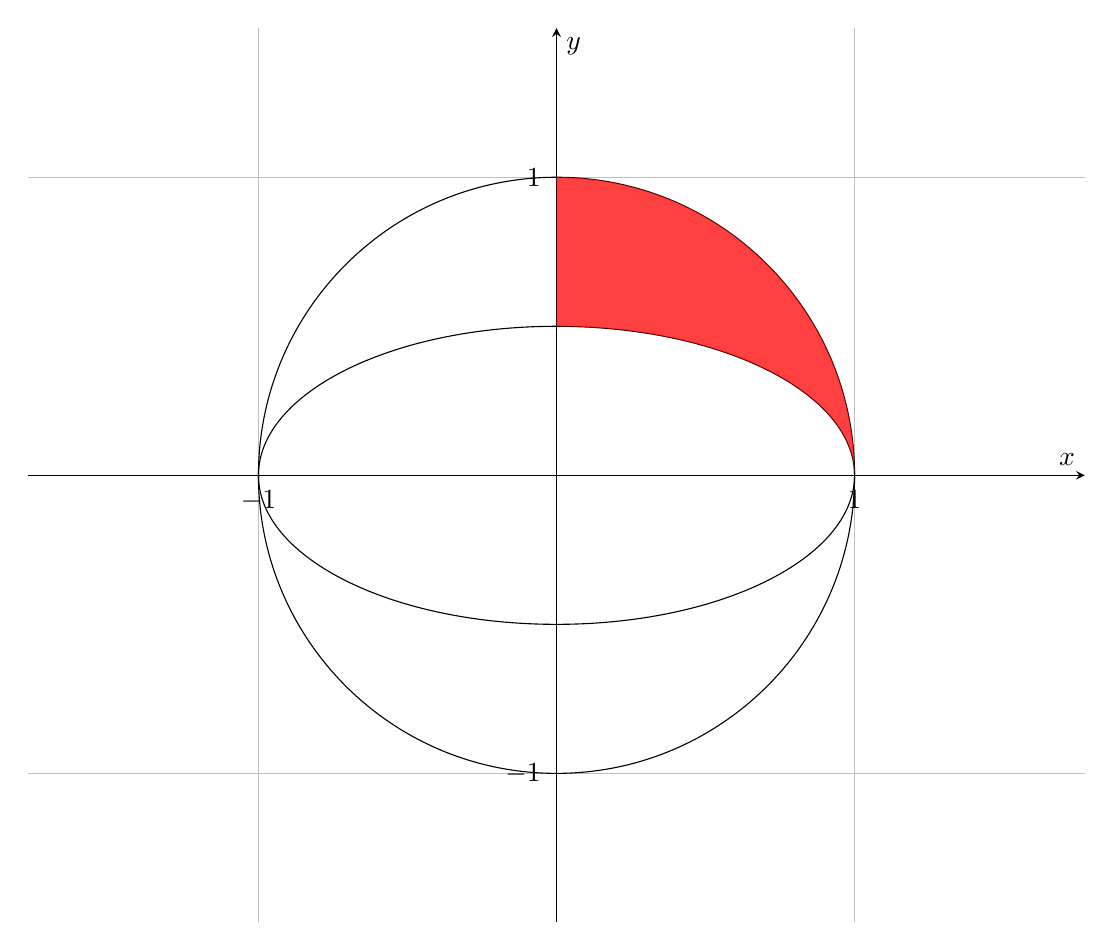
\begin{tikzpicture}[scale=1]
            \begin{axis}[
                    width=15cm,
                    xmin=-1.5,xmax=1.5,
                    xtick distance=1,
                    xlabel = $x$,
                    ymin=-1.5,ymax=1.5,
                    ytick distance=1,
                    ylabel = $y$,
                    axis equal,
                    grid=both,
                    axis lines = middle,
                    disabledatascaling
                ]
                %\draw [name path=A] (axis cs:0,-2) arc[start angle=-90, end angle=90, radius={transformdirectionx(2)}];
                %\draw [name path=B] (axis cs:0,-3) arc[start angle=-90, end angle=90, radius={transformdirectionx(3)}];

                \draw [name path=A1] (axis cs:1,0) arc[start angle=0, end angle=180, radius={transformdirectionx(1)}];
                \draw [name path=A2] (axis cs:-1,0) arc[start angle=180, end angle=360, radius={transformdirectionx(1)}];
                %\draw [name path=B] (axis cs:0,0) circle [x radius=1, y radius=1/4];

                \draw [name path=B1] (axis cs:1,0) arc(0:180:1 and 1/2);
                \draw [name path=B2] (axis cs:-1,0) arc(180:360:1 and 1/2);

                \tikzfillbetween[of=A1 and B1, soft clip={domain=0:1}]{red, opacity=0.75};
                %\tikzfillbetween[of=A2 and B2]{red, opacity=0.5};
            \end{axis}
        \end{tikzpicture}
    \end{center}

    Wir sehen, dass die Ellipsengleichung die untere und die Kreisgleichung die obere Schranke bilden.
    Damit formen wir unser Integrationsgebiet wie folgt um:
    $$
        A = \left\{(x, y) \in \R^2 \mid 0 \leq x \leq 1, \frac{\sqrt{1-x^2}}{2} \leq y \leq \sqrt{1-x^2} \right\}
    $$
\end{example}

\begin{example}{Integration über kartesische krummlinige Bereiche (Fortsetzung)}
    Dann können wir wie folgt die Fläche berechnen:
    $$
        \begin{aligned}
            \int\int_A (x+y) \d x \d y & = \int^1_0\int^{\sqrt{1-x^2}}_{\frac{\sqrt{1-x^2}}{2}} (x+y) \d y \d x                                                                                                       \\
                                       & = \int^1_0 \left[xy + \frac{y^2}{2}\right]^{\sqrt{1-x^2}}_{\frac{\sqrt{1-x^2}}{2}}  \d x                                                                                     \\
                                       & = \int^1_0 \left(x\sqrt{1-x^2} + \frac{1-x^2}{2} - \left( \frac{x\sqrt{1-x^2}}{2} - \frac{1-x^2}{8}\right)\right)  \d x                                                      \\
                                       & = \int^1_0 \left(\frac{x\sqrt{1-x^2}}{2} + \frac{3(1-x^2)}{8}\right)  \d x                                                                                                   \\
                                       & = \frac{1}{2}\int^1_0 x\sqrt{1-x^2} \d x + \frac{3}{8} \int^1_0 (1-x^2) \d x                                                                                                 \\
                                       & \overset{\footnote{$u = 1-x^2 \implies \frac{\d u}{\d x} = -2x \iff \d x = -\frac{\d u}{2x}$}}{=} -\frac{1}{4}\int^1_{x=0} \sqrt{u} \d u + \frac{3}{8} \int^1_0 (1-x^2) \d x \\
                                       & = -\frac{1}{4} \left[ \frac{2\sqrt{1-x^2}}{3} \right]^1_{0} + \frac{3}{8} \int^1_0 (1-x^2) \d x                                                                              \\
                                       & = \frac{1}{6} + \frac{3}{8} \int^1_0 (1-x^2) \d x                                                                                                                            \\
                                       & = \frac{1}{6} + \frac{3}{8} \left[ x-\frac{x^3}{3} \right]^1_0                                                                                                               \\
                                       & = \frac{1}{6} + \frac{3}{8} \left( 1-\frac{1}{3} \right)                                                                                                                     \\
                                       & = \frac{5}{12}                                                                                                                                                               \\
        \end{aligned}
    $$\qed
\end{example}

\begin{algo}{Schwerpunkt einer Grundfläche eines homogenen Gebietes}
    Der Schwerpunkt mit den Schwerpunktskoordinaten $(x_s, y_s)$ einer Fläche mit homogener Dichte ergibt sich mit der Flächenmaßzahl $F$ aus
    $$
        x_s = \frac{1}{F}\int_A x \d A \quad \land \quad y_s = \frac{1}{F}\int_A y \d A
    $$
\end{algo}

\begin{algo}{Masse einer Grundfläche eines inhomogenen Gebietes}
    Wird die spezifische Dichte eines Stoffes in der Koordinate $(x, y)$ gegeben durch $\rho(x, y)$, so lässt sich die Masse einer Fläche $A$ berechnen mit
    $$
        M = \int_A  \rho(x, y) \d A
    $$
\end{algo}

\begin{algo}{Integration in Polarkoordinaten}
    Bei der Umwandlung der kartesischen Koordinaten $(x, y)$ in \emph{Polarkoordinaten} umwandeln, gilt
    $$
        f(x, y) = f(r\cos\phi, r\sin\phi)\quad \land \quad \d y \d x = r \d r \d \phi
    $$

    Und dann insgesamt für die Integration:
    $$
        \int_A f(x, y) \d y \d x = \int_A f(r \cos\phi, r\sin\phi)r\d r\d\phi
    $$
\end{algo}

\begin{algo}{Uneigentliche Integrale mithilfe von Polarkoordinaten}
    Der Übergang zu Polarkoordinaten kann bei der Berechnung von uneigentlichen zweidimensionalen Integralen behilflich sein.
    Dabei gilt:
    $$
        \int_{x=-\infty}^\infty\int_{y=-\infty}^\infty f(x, y) \d y \d x = \int_{\phi = 0}^{2\pi} \int_{r = 0}^\infty f(r\cos\phi, r\sin\phi)r\d r\d\phi
    $$
\end{algo}

\begin{example}{Uneigentliche Integrale mithilfe von Polarkoordinaten}
    Berechnen Sie das folgende Integral
    $$
        \int_A x\cdot y \d A
    $$
    über dem Integrationsgebiet $A$ gegeben durch die Ungleichungen
    $$
        -2 \leq y \leq 2, \quad x \geq 0, \quad x^2 + y^2 \leq 4
    $$
    \begin{enumerate}[a)]
        \item in kartesischen Koordinaten,
        \item in Polarkoordinaten.
    \end{enumerate}

    \exampleseparator

    \begin{enumerate}[a)]
        \item
              Es gilt:
              $$
                  \begin{aligned}
                      \int_A x\cdot y \d A & = \int_{-2}^2 \int^{\sqrt{4-y^2}}_0 x\cdot y \d x \d y             \\
                                           & = \int_{-2}^2 y \left[ \frac{x^2}{2} \right]^{\sqrt{4-y^2}}_0 \d y \\
                                           & = \int_{-2}^2 \frac{y(4-y^2)}{2} \d y                              \\
                                           & = \frac{1}{2}\int_{-2}^2 (4y-y^3) \d y                             \\
                                           & = \frac{1}{2}\int_{-2}^2 (4y-y^3) \d y                             \\
                                           & = \frac{1}{2}\left[2y^2-\frac{y^4}{4}\right]_{0}^2                 \\
                                           & = 0
                  \end{aligned}
              $$\qed
    \end{enumerate}
\end{example}


\begin{example}{Uneigentliche Integrale mithilfe von Polarkoordinaten (Fortsetzung)}
    \begin{enumerate}[a)]
        \setcounter{enumi}{1}
        \item
              Es gilt:
              $$
                  \begin{aligned}
                      \int_A x\cdot y \d A & = \int^\frac{\pi}{2}_{-\frac{\pi}{2}} \int^2_0 r^3\cos\phi\sin\phi \d r \d \phi                                                                                             \\
                                           & = \int^\frac{\pi}{2}_{-\frac{\pi}{2}} \cos\phi\sin\phi \int^2_0 r^3 \d r \d \phi                                                                                            \\
                                           & = \int^\frac{\pi}{2}_{-\frac{\pi}{2}} \cos\phi\sin\phi \left[\frac{r^4}{4}\right]^2_0 \d \phi                                                                               \\
                                           & = 4\int^\frac{\pi}{2}_{-\frac{\pi}{2}} \cos\phi\sin\phi \d \phi                                                                                                             \\
                                           & \overset{\footnote{$u = \cos\phi \implies \frac{\d u}{\d \phi} = -\sin\phi \iff \d \phi = -\frac{\d u}{\sin \phi}$}}{=} -4\int^\frac{\pi}{2}_{\phi = -\frac{\pi}{2}} u \d u \\
                                           & = -4 \left[ \frac{\cos^2\phi}{2} \right]^\frac{\pi}{2}_{-\frac{\pi}{2}}                                                                                                     \\
                                           & = 0
                  \end{aligned}
              $$\qed
    \end{enumerate}
\end{example}
\subsection{Dreifachintegrale}

\begin{defi}{Dreifachintegral}
    Bezeichnet $V$ den Quader $\interval{x_0, x_1} \times \interval{y_0, y_1} \times \interval{z_0, z_1}$, so ist das \emph{Dreifachintegral} von $f$ über das Gebiet $V$ gegeben mit
    $$
        \int^{x_1}_{x_0}\int^{y_1}_{y_0}\int^{z_1}_{z_0} f(x, y, z) \d z\d y\d x = \int_A f \d A = \int\int\int_A f \d A
    $$
\end{defi}

\begin{bonus}{Volumenberechnung im $\R^3$}
    Die Berechnung eines Volumen $V$ über den Bereich $V'$ im $\R^3$ geschieht völlig analog zum $\R^2$:
    $$
        V = \int_{V'} 1 \d V'
    $$
\end{bonus}

\begin{bonus}{Schwerpunktberechnung im $\R^3$}
    Die Berechnung des Schwerpunktes $(x_s, y_s, z_s)$ mit Volumen $V$ über den Bereich $V'$ im $\R^3$ geschieht völlig analog zum $\R^2$:
    $$
        x_s = \frac{1}{V}\int_{V'} x \d V' \quad \land \quad y_s = \frac{1}{V}\int_{V'} y \d V' \quad \land \quad z_s = \frac{1}{V}\int_{V'} z \d V'
    $$
\end{bonus}

\begin{bonus}{Rechnen mit Kugelkoordinaten}
    Der Übergang zu Kugelkoordinaten kann bei der Berechnung von dreidimensionalen Integralen behilflich sein.
    Dabei gilt:
    $$
        \int\int\int f(x,y,z) \d z\d y\d x = \int\int\int f(r\cos\phi\sin\theta, r\sin\phi\sin\theta, r\cos\theta) \abs{r^2\sin\theta} \d\theta\d\phi\d r
    $$
\end{bonus}

\section{(*) Wachstums- und Zerfallsprozesse}

\subsection{Ungebremstes Wachstum}

\begin{defi}{Diskretes ungebremstes Wachstum}
    Gegeben sei ein Wachstum $k$ innerhalb einer (beliebigen) Zeiteinheit $\Delta t_0$, eine Startpopulation $y_0$ und eine Änderungsrate
    $$
        \Delta y = k\cdot y
    $$
    dann ist die Lösungsfunktion
    $$
        \boxed{y_n = y_0\cdot (1+k)^n}
    $$
    wobei $y_n = y(n\cdot \Delta t_0)$ den Zustand nach $n$ Zeitschritten der Länge $\Delta t_0$ angibt.
\end{defi}

\begin{bonus}{Diskretes ungebremstes Wachstum für Zeitteile}s
    Gegeben sei ein Wachstum $k$ innerhalb einer (beliebigen) Zeiteinheit $\Delta t_0 = 1$, eine Startpopulation $y_0$ und eine Änderungsrate
    $$
        \Delta y = k_{\Delta t_0}\cdot y
    $$

    Betrachten wir nun einen \emph{Zeitteil} $\Delta t$, dann ist das modifizierte Modell
    $$
        \Delta y = y_n - y_{n-1} = k_{\Delta t}\cdot  y_{n-1}\cdot  \Delta t
    $$
    mit der Lösung
    $$
        \boxed{y_n = y_0\cdot (1 + k_{\Delta t} \cdot \Delta t)^n}
    $$
    wobei $y_n = y(n\cdot \Delta t)$ den Zustand nach $n$ Zeitschritten der Länge $\Delta t$ angibt.

    Die Lösung dieses Modells wird auch als \emph{diskrete Evolutionsgleichung des ungebremsten Wachstums} bezeichnet.
\end{bonus}

\begin{defi}{Kontinuierliches Modell der Evolutionsgleichung}
    Zur Lösung der Modellgleichung
    $$
        \lim_{\Delta t \to 0} \frac{\Delta y}{\Delta t} = k\cdot y
    $$
    mit $y(0) = y_0$ und $k$ (kontinuierliches) Wachstum, so ist die \emph{kontinuierliche} Lösungsfunktion
    $$
        \boxed{y(t) = y_o \cdot e^{kt}}
    $$
    und wegen $\Delta t \to 0$ ist dies gleichbedeutend zu
    $$
        y'(t) = k \cdot y(t) \ \text{mit} \ y(0) = 0
    $$

    Ein solches Problem heißt \emph{Differentialgleichung mit Anfangswert} oder \emph{Anfangswertproblem}.
\end{defi}

\subsection{Gebremstes Wachstum - Störung erster Ordnung}

\begin{defi}{Diskretes Modell des Wachstums mit Störung erster Ordnung}
    Gegeben sei ein Wachstum $k$ innerhalb einer (beliebigen) Zeiteinheit $\Delta t_0$, eine Startpopulation $y(0) = y_0$, $\Delta t$ ein Zeitteil, $a$ die \emph{Abnahme pro Zeiteinheit} und eine Änderungsrate
    $$
        \Delta y = (k\cdot y - a) \cdot \Delta t
    $$
    dann ist die Lösungsfunktion
    $$
        \boxed{y_n = \left( y(0) - \frac{a}{k} \right) \cdot \left( 1 + k \cdot \Delta t \right)^n + \frac{a}{k}}
    $$
\end{defi}

\begin{defi}{Kontinuierliches Modell des Wachstums mit Störung erster Ordnung}
    Zur Lösung der Modellgleichung
    $$
        \lim_{\Delta t \to 0} \frac{\Delta y}{\Delta t} = k\cdot y - a
    $$
    mit $y(0) = y_0$, $k$ (kontinuierliches) Wachstum und $a$ \emph{kontinuierliche Abnahme} pro Zeiteinheit, ist die \emph{kontinuierliche} Lösungsfunktion
    $$
        \boxed{y(t) = \left( y(0) - \frac{a}{k} \right) \cdot e^{kt} + \frac{a}{k}}
    $$
    und wegen $\Delta t \to 0$ ist dies gleichbedeutend zu
    $$
        y'(t) = k \cdot y(t) - a
    $$
\end{defi}

\begin{defi}{Stationäre Lösung}
    Die konstanten Werte, ermittelt durch $\Delta y = 0$, heißen \emph{stationäre Lösungen} $y_s$.

    Für Wachstumsmodelle mit Störung erster Ordnung gilt:
    $$
        y_s = \frac{a}{k}
    $$
\end{defi}

\subsection{Logistisches Wachstum - Störung zweiter Ordnung}

\begin{defi}{Diskretes Modell des Wachstums mit Störung zweiter Ordnung}
    Gegeben sei ein Wachstum $k$ innerhalb einer (beliebigen) Zeiteinheit $\Delta t_0$, eine Startpopulation $y(0) = y_0$, $\Delta t$ ein Zeitteil, $R$ \emph{Oberschranke der verfügbaren Ressourcen} und eine Änderungsrate
    $$
        \Delta y = (k\cdot y \cdot (R-y)) \cdot \Delta t
    $$
    dann ist die Lösungsfunktion
    $$
        \boxed{y_n = \frac{R}{\frac{R-y_0}{y_0} \cdot (1 + R \cdot k \cdot \Delta t)^{-n} + 1}}
    $$
\end{defi}

\begin{defi}{Kontinuierliches Modell des Wachstums mit Störung zweiter Ordnung}
    Zur Lösung der Modellgleichung
    $$
        \lim_{\Delta t \to 0} \frac{\Delta y}{\Delta t} = k\cdot y \cdot (R-y)
    $$
    mit $y(0) = y_0$, $k$ (kontinuierliches) Wachstum und $R$ \emph{Oberschranke der verfügbaren Ressourcen}, ist die \emph{kontinuierliche} Lösungsfunktion
    $$
        \boxed{y(t) = \frac{R}{\frac{R-y_0}{y_0} \cdot e^{-Rkt} + 1}}
    $$
    und wegen $\Delta t \to 0$ ist dies gleichbedeutend zu
    $$
        y'(t) = k \cdot y(t) \cdot (R-y(t))
    $$
\end{defi}

\section{Gewöhnliche Differentialgleichungen}

\begin{defi}{Gewöhnliche Differentialgleichung $n$-ter Ordnung}
    Eine Gleichung der Form
    $$
        y^{(n)} = f(x, y, y', y'', \ldots, y^{(n-1)})
    $$
    heißt \emph{(explizite) gewöhnliche Differentialgleichung n-ter Ordnung}.

    Ist die Gleichung in der Form
    $$
        f(x, y, y', y'', \ldots, y^{(n)}) = 0
    $$
    gegeben, so heißt die Differentialgleichung \emph{implizit}.

    Erfüllt $y(x)$ die Differentialgleichung, so heißt $y$ \emph{allgemeine Lösung der Differentialgleichung}.
\end{defi}

\begin{defi}{Anfangswertproblem}
    Die Vorgabe einer expliziten Differentialgleichung und der Werte
    $$
        x_0, \quad y(x_0) = y_0, \quad y'(x_0) = y_1, \quad \ldots, \quad y^{(n-1)}(x_0) = y_{n-1}
    $$
    heißt \emph{Anfangswertproblem}.

    Erfüllt $y(x)$ das Anfangswertproblem, so heißt $y$ \emph{spezielle Lösung des Anfangswertproblems}.
\end{defi}

\subsection{Lösungsverfahren für Differentialgleichungen erster Ordnung}

\begin{algo}{Trennung der Variablen}
    Gegeben: Differentialgleichung der Form
    $$
        \boxed{y' = f(x) \cdot g(y)} \quad \iff \quad \frac{\d y}{\d x} = f(x) \cdot g(y)
    $$
    \begin{enumerate}
        \item $x$ und $y$ wie folgt trennen:
              $$
                  \frac{1}{g(y)} \d y = f(x) \d x
              $$
        \item Integration liefert:
              $$
                  \int \frac{1}{g(y)} \d y = \int f(x) \d x
              $$
        \item Umstellen nach $y$ liefert die Lösung der Differentialgleichung
    \end{enumerate}
\end{algo}

\begin{example}{Trennung der Variablen}
    Berechnen Sie die allgemeine Lösung der Differentialgleichung
    $$
        y' + (1+x)\cdot y = 0\quad \iff \quad y' = -y\cdot (1+x)
    $$
    \exampleseparator

    $$
        \begin{aligned}
                       & \frac{\d y}{\d x}      &  & = -y \cdot (1+x)                        \\
            \iff \quad & -\frac{1}{y} \d y      &  & = (1+x) \d x                            \\
            \iff \quad & \int -\frac{1}{y} \d y &  & = \int (1+x) \d                         \\
            \iff \quad & - \ln\abs{y} - c_2     &  & = x + \frac{x^2}{2} + c_1               \\
            \iff \quad & y                      &  & = e^{-(c_1 + c_2)}e^{-\frac{x}{2}(x+2)} \\
            \iff \quad & y                      &  & = ce^{-\frac{x}{2}(x+2)}                \\
        \end{aligned}
    $$\qed
\end{example}

\begin{algo}{Substitution}
    \begin{itemize}
        \item Differentialgleichung vom Typ
              $$
                  \boxed{y' = f(ax + by + c)}
              $$
              \begin{enumerate}
                  \item Substituiere $z = ax + by + c$
                  \item Es ergibt sich
                        $$
                            y = \frac{z -ax - c}{b} \quad \implies \quad y' = \frac{z' - a}{b}
                        $$
                        bzw.
                        $$
                            z' = a + bf(z)
                        $$
                  \item Lösen mithile von \emph{Trennung der Variablen} (\emph{Tipp:} Dividieren durch rechte Seite)
                  \item Rücksubstitution in $y = \frac{z -ax - c}{b}$ ergibt die Lösung
              \end{enumerate}
        \item Differentialgleichung vom Typ
              $$
                  \boxed{y' = f\left(\frac{y}{x}\right)}
              $$
              \begin{enumerate}
                  \item Substituiere $z = \frac{y}{x}$
                  \item Es ergibt sich (Produktregel!)
                        $$
                            y = z \cdot x \quad \implies \quad y' = z + z' \cdot x
                        $$
                        bzw.
                        $$
                            z' = \frac{f(z) - z}{x} \quad \iff \quad z + z' \cdot x = f(z)
                        $$
                  \item Lösen mithile von \emph{Trennung der Variablen}
                  \item Rücksubstitution in $y = z \cdot x$ ergibt die allgemeine Lösung
              \end{enumerate}
    \end{itemize}
\end{algo}

\begin{example}{Substitution}
    Lösen Sie die folgende Differentialgleichung mit Hilfe einer geeigneten Substitution ($x \neq 0$):
    $$
        y' = \frac{1}{\sin\left(\frac{y}{x}\right)} + \frac{y}{x}
    $$
    \exampleseparator

    Sei $u = \frac{y}{x}$ ($\implies u' = \frac{xy' - y}{x^2} \iff y' = u + xu'$). Dann gilt:

    $$
        \begin{aligned}
                       & y'                  &  & = \frac{1}{\sin\left(\frac{y}{x}\right)} + \frac{y}{x} \\
            \iff \quad & u + xu'             &  & = \frac{1}{\sin u} + u                                 \\
            \iff \quad & xu'                 &  & = \frac{1}{\sin u}                                     \\
            \iff \quad & \frac{x \d u}{\d x} &  & = \frac{1}{\sin u}                                     \\
            \iff \quad & \sin u \d u         &  & = \frac{1}{x} \d x                                     \\
            \iff \quad & \int \sin u \d u    &  & = \int \frac{1}{x} \d x                                \\
            \iff \quad & -\cos (u) + c_2     &  & = \ln\abs{x} + c_1                                     \\
            \iff \quad & \cos (u)            &  & = -\ln\abs{x} - c_1 + c_2                              \\
            \iff \quad & u                   &  & = \arccos(-\ln\abs{x} - c_1 + c_2)                     \\
            \iff \quad & \frac{y}{x}         &  & = \arccos(-\ln\abs{x} - c_1 + c_2)                     \\
            \iff \quad & y                   &  & = x\arccos(c - \ln\abs{x})                             \\
        \end{aligned}
    $$\qed
\end{example}

\begin{defi}{Lineare Differentialgleichung}
    Die Gleichung
    $$
        y' + f(x) \cdot y = 0
    $$
    heißt \emph{linear homogene Differentialgleichung} 1. Ordung.

    Die Gleichung
    $$
        y' + f(x) \cdot y = g(x)
    $$
    heißt \emph{linear inhomogene Differentialgleichung} 1. Ordung und
    $g(x)$ heißt \emph{Störfunktion}.

    Das zugehörige Anfangswertproblem heißt \emph{lineares Anfangswertproblem}.
\end{defi}

\begin{algo}{Lösen von linearen homogenen Differentialgleichungen 1. Ordnung}
    Für eine Gleichung
    $$
        \boxed{y' + f(x)\cdot y = 0}
    $$
    ist die allgemeine Lösung
    $$
        y = ce^{\int -f(x) \d x}
    $$

    $c$ wird dann durch Einsetzen eines Anfangswertes berechnet.
\end{algo}

\begin{algo}{Variation der Konstanten}
    Gegeben: Differentialgleichung der Form
    $$
        \boxed{y' + f(x)\cdot y = g(x)}
    $$
    \begin{enumerate}
        \item Löse homogene Differentialgleichung mit
              $$
                  y = ce^{\int - f(x) \d x}
              $$
        \item Ersetze $c$ durch $c(x)$
        \item Berechne $y'$
        \item Vergleiche $y'$ mit ursprünglicher Störfunktion
        \item Bestimme aus der Differentialgleichung die Lösung für $c(x)$ (enthält neue Konstante!)
        \item Einsetzen in
              $$
                  y = c(x) \cdot e^{\int - f(x) \d x}
              $$
              ergibt die allgemeine Lösung
    \end{enumerate}
\end{algo}

\begin{example}{Variation der Konstanten}
    Berechnen Sie die allgemeine Lösung der Differentialgleichung
    $$
        (x-2) \cdot y' = y + 2(x-2)^3
    $$
    \exampleseparator

    Umwandeln in allgemeine Darstellung:
    $$
        (x-2) \cdot y' = y + 2(x-2)^3 \quad \iff \quad y' = \frac{y}{x-2} + 2(x-2)^2 \quad \iff \quad y' - \frac{1}{x-2}\cdot y = 2(x-2)^2
    $$
    Lösen der homogenen Gleichung:
    $$
        \begin{aligned}
                       & y'_h - \frac{1}{x-2}\cdot y_h &  & = 0                         \\
            \iff \quad & y'_h                          &  & = \frac{1}{x-2}\cdot y_h    \\
            \iff \quad & \frac{1}{y_h} \d y_h          &  & = \frac{1}{x-2}\d x         \\
            \iff \quad & \int \frac{1}{y_h} \d y_h     &  & = \int \frac{1}{x-2}\d x    \\
            \iff \quad & \ln(y_h) + c_2                &  & = \ln (x-2) + c_1           \\
            \iff \quad & (y_h)                         &  & = e^{\ln (x-2) + c_1 - c_2} \\
            \iff \quad & y_h                           &  & = c(x-2)                    \\
        \end{aligned}
    $$

    Lösen der Störfunktion:
    $$
        \begin{aligned}
                           & y  &  & = c(x) \cdot (x-2)  \\
            \implies \quad & y' &  & = c'(x)(x-2) + c(x)
        \end{aligned}
    $$
    $$
        \begin{aligned}
                       & y' - \frac{1}{x-2}\cdot y                                                                  &  & = 2(x-2)^2                   \\
            \iff \quad & \underbrace{c'(x)(x-2) + c(x)}_{y'} - \frac{1}{x-2}\cdot \underbrace{c(x) \cdot (x-2)}_{y} &  & = 2(x-2)^2                   \\
            \iff \quad & c'(x)(x-2)                                                                                 &  & = 2(x-2)^2                   \\
            \iff \quad & c'(x)                                                                                      &  & = 2(x-2)                     \\
            \iff \quad & \int 1 \d c                                                                                &  & = 2\int x\d x - 4\int 1 \d x \\
            \iff \quad & c(x)                                                                                       &  & = x^2 - 4x + c_1
        \end{aligned}
    $$

    Damit erhalten wir insgesamt:
    $$
        y = (x^2 - 4x + c)(x-2) = c(x-2) + (x-4)(x-2)x
    $$\qed
\end{example}

\begin{defi}{Superpositionsprinzip (inhomogene lineare Differentialgleichungen)}
    Die Lösung einer \emph{inhomogenen linearen Differentialgleichung} setzt sich zusammen aus der allgemeinen Lösung der homogenen Differentialgleichung $y_h$ und einer partikulären Lösung der \emph{inhomogenen Differentialgleichung} $y_p$
    $$
        y = y_h + y_p
    $$
\end{defi}

\begin{algo}{Ansatz vom Typ der rechten Seite}
    Man rät eine Lösung, indem man einen Ansatz für $y_p$ vom Typ der Störfunktion $g(x)$ wählt:

    \begin{center}
        \begin{tabular}{c | c l}
            Störfunktion $g(x)$            & Ansatz für $y_p$                                                                        \\
            \hline
            $c_0$                          & $\lambda_0$                                        & \rdelim\}{3}{3mm}[polynomiell]     \\
            $c_0 + c_1x$                   & $\lambda_0 + \lambda_1 x$                                                               \\
            $c_0 + c_1x + \ldots + c_nx^n$ & $\lambda_0 + \lambda_1 x + \ldots + \lambda_nx^n$                                       \\
            \hline
            $c_0e^{ax}$                    & $\lambda_0 e^{ax}$                                 & \rdelim\}{4}{3mm}[exponentiell]    \\
            $c_0e^{ax}$                    & $\lambda_0 xe^{ax}$                                                                     \\
            $c_0e^{ax}$                    & $\ldots$                                                                                \\
            $c_0e^{ax}$                    & $\lambda_0 x^ne^{ax}$                                                                   \\
            \hline
            $c_0\sin(ax) + c_1\cos(ax)$    & $\lambda_0\sin(ax) + \lambda_1\cos(ax)$            & \rdelim\}{3}{3mm}[trigonometrisch] \\
            $c_0e^{ax}\cdot \sin(bx)$      & $x\cdot (\lambda_1 \sin(bx) + \lambda_2 \cos(bx))$                                      \\
            $c_0e^{ax}\cdot \cos(bx)$      & $x\cdot (\lambda_1 \sin(bx) + \lambda_2 \cos(bx))$                                      \\
        \end{tabular}
    \end{center}

    \emph{Bemerkungen:}
    \begin{itemize}
        \item Bei einer Summe von mehreren Funktionstypen sollten entsprechend viele partikuläre Teillösungen berechnet werden. Die Summe dieser Teillösungen entspricht dann insgesamt der partikulären Lösung $y_p$.
        \item Existiert für eine Störfunktion $g(x) = cx^ne^{ax}$ ein Term $\mu x^ne^{ax}$ bereits in der homogenen Lösung, wählt man als Ansatz für $y_p = \lambda x^{n+1}e^{ax}$ (siehe Beispiel).
    \end{itemize}
\end{algo}

\begin{example}{Ansatz vom Typ der rechten Seite}
    Berechnen Sie die allgemeine Lösung der linearen Differentialgleichung
    $$
        y'- y = 9e^x
    $$
    \exampleseparator

    Lösen der homogenen Gleichung:
    $$
        y_h'- y_h = 0 \implies y_h = ce^{x}
    $$

    Mit der partikulären Lösung ($y_p = c_0xe^{x}$)
    $$
        y_p = c_0xe^x \implies y'_p = c_0(e^x + xe^x)
    $$
    gilt dann:
    $$
        \begin{aligned}
                           & y'- y                     &  & = 9e^x \\
            \iff \quad     & c_0(e^x + xe^x) - c_0xe^x &  & = 9e^x \\
            \iff \quad     & c_0e^x(1 + x - x)         &  & = 9e^x \\
            \implies \quad & c_0                       &  & = 9
        \end{aligned}
    $$

    Und schlussendlich:
    $$
        y = y_h + y_p \implies y = ce^x + 9e^xx
    $$\qed
\end{example}

\begin{algo}{Bernoulli-Differentialgleichung}
    Gegeben: Differentialgleichung der Form
    $$
        \boxed{y' + f(x) \cdot y = g(x)\cdot y^\alpha}
    $$
    \begin{enumerate}
        \item Substituiere
              $$
                  z = y^{1-\alpha} \quad \iff \quad y = z^{\frac{1}{1-\alpha}}
              $$
        \item Einsetzen in die Differentialgleichung ergibt
              $$
                  z' + (1-\alpha) \cdot f(x)\cdot z = g(x) \cdot (1-\alpha)
              $$
        \item Lösen der linearen Differentialgleichung
        \item Rücksubstitution in
              $$
                  y = z^{\frac{1}{1-\alpha}}
              $$
              ergibt die allgemeine Lösung
    \end{enumerate}
\end{algo}

\begin{defi}{Exakte Differentialgleichung}
    Eine Differentialgleichung der Form
    $$
        p(x, y) + q(x, y) \cdot y' = 0 \quad \iff \quad p(x, y) \d x + q(x, y) \d y = 0
    $$
    mit
    $$
        p_y = q_x \ \text{\emph{(Integrabilitätsbedingung)}}
    $$
    heißt \emph{exakte Differentialgleichung}.
\end{defi}

\begin{algo}{Lösen von exakten Differentialgleichungen}
    Gegeben: Differentialgleichung der Form
    $$
        \boxed{p(x, y) + q(x, y) \cdot y' = 0 \quad \iff \quad p(x, y) \d x + q(x, y) \d y = 0}
    $$
    \begin{enumerate}
        \item Prüfen der Integrabilitätsbedingung
              $$
                  p_y = q_x
              $$
        \item Stammfunktion berechnen mit
              $$
                  \underbrace{F(x, y) = \int p \d x}_{(*)} \quad \text{oder} \quad \underbrace{F(x, y) = \int q \d y}_{(**)}
              $$
              \subitem Konstante $c$ ersetzen mit $c(y)$ $(*)$ bzw. $c(x)$ $(**)$
        \item Differentiation von $F(x, y)$ nach $y$ $(*)$ bzw. nach $x$ $(**)$
        \item Es ergibt sich
              $$
                  c(y)' = f(y) \quad \implies c(y) = \int f(y) \d y \quad (*)
              $$
              bzw.
              $$
                  c(x)' = f(x) \quad \implies c(x) = \int f(x) \d x \quad (**)
              $$
        \item Einsetzen ergibt die allgemeine Lösung
    \end{enumerate}
\end{algo}

\begin{defi}{Integrierender Faktor (Euler-Multiplikator)}
    $\mu(x, y)$ ist genau dann ein \emph{integrierender Faktor} oder \emph{Euler-Multiplikator} für eine Funktion
    $$
        p(x, y) + q(x, y) \cdot y' = 0 \quad \iff \quad p(x, y) \d x + q(x, y) \d y = 0
    $$
    wenn die Integrabilitätsbedingung
    $$
        \frac{\partial \mu p}{\partial y} = \frac{\partial \mu q}{\partial x}
    $$
    erfüllt wird.
\end{defi}

\begin{algo}{Lösen von Differentialgleichungen mithilfe eines integrierenden Faktors}
    Gegeben: Differentialgleichung der Form
    $$
        \boxed{p(x, y) + q(x, y) \cdot y' = 0 \quad \iff \quad p(x, y) \d x + q(x, y) \d y = 0}
    $$
    bei der die \emph{Integrabilitätsbedingung nicht erfüllt} wird.

    Wir betrachten hier nur integrierende Faktoren, die nur von $x$ bzw. nur von $y$ abhängig sind.

    \begin{enumerate}
        \item Integrierender Faktor ist gegeben mit
              $$
                  \underbrace{\mu(x) = e^{\int m(x) \d x}}_{(*)} \quad \text{oder} \quad \underbrace{\mu(y) = e^{\int m(y) \d y}}_{(**)}
              $$
              \subitem $(*)$ Untersuchen, ob $\mu$ nur von $x$ abhängt:
              $$
                  m(x) = \frac{p_y - q_x}{q}
              $$
              \subitem $(**)$ Untersuchen, ob $\mu$ nur von $y$ abhängt:
              $$
                  m(y) = \frac{q_x - p_y}{p}
              $$
        \item $m$ in entsprechende Formel für $\mu$ einsetzen
        \item Einsetzen in die Differentialgleichung liefert
              $$
                  \mu p(x, y) + \mu q(x, y) \cdot y' = 0 \quad \iff \quad \mu p(x, y) \d x + \mu q(x, y) \d y = 0
              $$
        \item Prüfen der Integrabilitätsbedingung
        \item Lösen der exakten Differentialgleichung
    \end{enumerate}
\end{algo}

\begin{example}{Lösen von Differentialgleichungen mithilfe eines integrierenden Faktors}
    Lösen Sie die Differentialgleichung
    $$
        (3xy + 2y^2) + (x^2 + 2xy) y' = 0
    $$

    \exampleseparator

    Es gilt:
    $$
        (3xy + 2y^2) + (x^2 + 2xy) y' = 0 \quad \iff \quad \underbrace{(3xy + 2y^2)}_{p(x, y)}\d x + \underbrace{(x^2 + 2xy)}_{q(x, y)}\d y = 0
    $$
    Integrabilitätsbedingung:
    $$
        p_y = 3x + 4y \quad \neq \quad 2x + 2y = q_x \quad \lightning
    $$

    Integrierenden Faktor (Euler-Multiplikator) $\mu(x) = e^{\int m(x) \d x}$ bzw. $\mu(y) = e^{\int m(y) \d y}$ bestimmen:
    \begin{itemize}
        \item Untersuchung, ob $\mu$ nur von $y$ abhängt:
              $$
                  m = \frac{q_x - p_y}{p} = \frac{2x + 2y - \left(3x + 4y\right)}{3xy + 2y^2} = \frac{-x - 2y}{3xy + 2y^2} \quad \lightning
              $$
        \item Untersuchung, ob $\mu$ nur von $x$ abhängt:
              $$
                  m = \frac{p_y - q_x}{q} = \frac{3x + 4y - (2x + 2y)}{x^2 + 2xy} = \frac{x + 2y}{x^2 + 2xy} = \frac{x+2y}{x(x+2y)} = \frac{1}{x} \quad \checkmark
              $$
    \end{itemize}

    Damit erhalten wir den integrierenden Faktor mit:
    $$
        \mu(x) = e^{\int \frac{1}{x} \d x} = cx \qquad (\text{sei} \ c = 1)
    $$
    Einsetzen in die DGL:
    $$
        \underbrace{\left(3x^2y + 2xy^2\right)}_{p(x, y)}\d x + \underbrace{\left(x^3 + 2x^2y\right)}_{q(x, y)}\d y = 0
    $$
    Integrabilitätsbedingung:
    $$
        p_y = 3x^2 + 4xy \quad = \quad 3x^2 + 4xy = q_x \quad \checkmark
    $$
    Wir wissen:
    $$
        \underbrace{F = \int q \d y = x^3y + x^2y^2 + c(x)}_{F_y = q} \implies \underbrace{3x^2y + 2xy^2 + c'(x) = 3x^2y + 2xy^2}_{F_x = p}  \implies  c(x) = c
    $$

    Und insgesamt gilt damit:
    $$
        F = x^3y + x^2y^2 + c
    $$\qed
\end{example}

\subsection{Lösungsverfahren für Differentialgleichungen zweiter Ordnung}

\begin{defi}{Charakteristische Gleichung}
    Die Gleichung
    $$
        \alpha^2 + a\alpha + b = 0
    $$
    heißt die zur Differentialgleichung
    $$
        y'' + ay' + b = 0
    $$
    gehörende \emph{charakteristische Gleichung}.
\end{defi}

\begin{bonus}{Superpositionsprinzip (homogene lineare Differentialgleichungen)}
    Sind $y_1(x)$ und $y_2(x)$ Lösungen einer \emph{homogenen linearen Differentialgleichung}, so ist auch jede \emph{Linearkombination}
    $$
        \lambda\cdot  y_1(x) + \mu\cdot  y_2(x)
    $$
    eine allgemeine Lösung der Differentialgleichung.
\end{bonus}

\begin{algo}{Lösen von linearen homogenen Differentialgleichungen 2. Ordnung}
    Für eine Gleichung
    $$
        \boxed{y'' + ay' + by = 0}
    $$
    stelle man die charakteristische Gleichung auf, mit
    $$
        \alpha^2 + a\alpha + b = 0 \quad \implies \quad \alpha = -\frac{a}{2} \pm \sqrt{\left(\frac{a}{2}\right)^2 - b}
    $$

    Dann gilt mit $D = \left(\frac{a}{2}\right)^2 - b$ (Diskriminante):
    \begin{itemize}
        \item $D > 0$:
              $$
                  y_h = \lambda_1 e^{\alpha_1 x} + \lambda_2 e^{\alpha_2 x}
              $$
        \item $D = 0$:
              $$
                  y_h = (\lambda_1 + \lambda_2x)\cdot  e^{\alpha x}
              $$
        \item $D < 0$:
              $$
                  y_h = e^{\Re(\alpha)} \cdot \left( \lambda_1 \cos(\Im(\alpha)) + \lambda_2 \sin(\Im(\alpha)) \right) = e^{-\frac{a}{2}} \cdot \left( \lambda_1 \cos(\sqrt{-D}) + \lambda_2 \sin(\sqrt{-D}) \right)
              $$
    \end{itemize}

    \emph{Bemerkung:}
    \begin{itemize}
        \item $\Re(\alpha)$ ist der Realteil der Nullstelle
        \item $\Im(\alpha)$ ist der Imaginärteil der Nullstelle
    \end{itemize}
\end{algo}

\begin{algo}{Lösen von linearen Differentialgleichungssystemen}
    Gegeben: Differentialgleichungssystem der Form
    \begin{equation}
        y'  = ay + bz
    \end{equation}
    \begin{equation}
        z'  = dy + cz
    \end{equation}

    \begin{enumerate}
        \item Umstellen von (1) nach $z$ ergibt
              $$
                  z = \frac{y' - ay}{b}
              $$
        \item Differentiation von (1) und anschließendes Einsetzen von $z$ ergibt
              $$
                  y'' - (a + c) \cdot y' + (ac -bd) \cdot y = 0
              $$
        \item Lösen der homogenen Differentialgleichung mit der charakteristischen Gleichung
              $$
                  \alpha^2 - (a+c)\alpha + (ac-bd) = 0
              $$
              ergibt dann die allgemeine Lösung für $y$
        \item Einsetzen von $y$ (und $y'$) in
              $$
                  z =  \frac{y' - ay}{b}
              $$
              ergibt die allgemeine Lösung für $z$
    \end{enumerate}
\end{algo}

\begin{example}{Lösen von linearen Differentialgleichungssystemen}
    Lösen Sie folgendes Differentialgleichungssystem:
    $$
        \begin{aligned}
            y' & = y + 2z          \\
            z' & = 2y + z - 2e^{x}
        \end{aligned}
    $$

    \exampleseparator

    Wir leiten $y'$ ab:
    $$
        \begin{aligned}
                       & y' = y + 2z \quad \iff \quad z = \frac{y'- y}{2} \\
            \iff \quad & y'' - y'  - 2z' = 0
        \end{aligned}
    $$
    Einsetzen von $z'$:
    $$
        y'' - y'  - 2z' = 0 \quad \iff \quad  y'' - y'  - 4y -2z + 4e^{x} = 0
    $$
    Einsetzen von $z$:
    $$
        \begin{aligned}
                       & y'' - y'  - 4y -2z + 4e^{x} = 0 \\
            \iff \quad & y'' - 2y'  - 3y  = -4e^{x}
        \end{aligned}
    $$

    Lösung der homogenen Gleichung:
    $$
        \begin{aligned}
                           & y'' - 2y'  - 3y  = 0                          \\
            \implies \quad & \alpha^2 - 2\alpha - 3 = 0                    \\
            \implies \quad & \alpha = 1 \pm \sqrt{\left( -1 \right)^2 + 3} \\
            \iff \quad     & \alpha = 1 \pm 2                              \\
            \implies \quad & y_h = \lambda_1e^{-x} + \lambda_2e^{3x}
        \end{aligned}
    $$

    Berechnen der partikulären Lösung:
    $$
        y_p = ce^x \quad \implies \quad y'_p = ce^x \quad \implies \quad y''_p = ce^x
    $$
    $$
        \begin{aligned}
                           & y''_p - 2y'_p  - 3y_p &  & = -4e^{x} \\
            \iff \quad     & ce^x - 2ce^x  - 3ce^x &  & = -4e^{x} \\
            \iff \quad     & -4ce^x                &  & = -4e^{x} \\
            \implies \quad & c = 1
        \end{aligned}
    $$
    Dann gilt insgesamt:
    $$
        y = y_h + y_p = \lambda_1e^{-x} + \lambda_2e^{3x} + e^x
    $$
    und
    $$
        z = \frac{y'- y}{2} = \frac{\left( -\lambda_1e^{-x} + 3\lambda_2e^{3x} + e^x \right) - \left( \lambda_1e^{-x} + \lambda_2e^{3x} + e^x \right)}{2} = \lambda_2e^{3x} - \lambda_1e^{-x}
    $$\qed
\end{example}

\printindex
\printindex[Beispiele]

\end{document}
